\documentclass[12pt]{article}
\frenchspacing
\usepackage[utf8x]{inputenc}
\usepackage[T2A]{fontenc}
\usepackage{amsmath}
\usepackage{amsfonts}
\usepackage{amssymb}
\usepackage[russian]{babel}
\usepackage{graphicx}
\usepackage{hyperref}
\usepackage{multirow}
\usepackage[left=2cm,right=2cm,top=2cm,bottom=2cm,bindingoffset=0cm]{geometry}
\author{Рашковецкий М.М., группа 526т}
\date{\today}
\title{Лабораторная работа 2.4.1\\Определение теплоты испарения жидкости}
\begin{document}
	\maketitle
	
	{\parindent=1cm \hangindent=1cm \parskip=0.5cm
	{\bfseries Цель работы:} измерение давления насыщенного пара жидкости при разной температуре; вычисление по полученным данным теплоты испарения жидкости по уравнению Клапейрона --- Клаузиуса.
	
	\hangindent=1cm
	{\bfseries Оборудование и материалы:} термостат; герметичный сосуд с исследуемой жидкостью; отсчётный микроскоп.\par}
	\section*{Краткая теория}
	
	\indent Непосредственное измерение теплоты парообразования очень неточно из-за неконтролируемых потерь тепла. Поэтому в работе используется косвенный метод, основанный на уравнении Клапейрона --- Клаузиуса:
	\begin{equation}
		\label{eq:klapeiron-klausius}
		\frac{dP}{dT}=\frac{L}{T \left( v_\text{п} - v_\text{ж} \right) },
	\end{equation}
	где $P$ --- давление насыщенного пара, $T$ --- температура, $L$ --- удельная или молярная теплота парообразования, $v_\text{п}$ и $v_\text{ж}$ --- удельные или молярные объёмы пара и жидкости соответственно.
	
	У большинства веществ $v_\text{п}$ на несколько порядков превышает $v_\text{ж}$, поэтому последним можно пренебречь, тогда первое обозначают просто $v$.
	
	Запишем для насыщенного пара уравнение Ван-дер-Ваальса:
	\begin{equation}
		\label{eq:van-der-vaals}
		\left( P + \frac{a}{v^2} \right) \left( v - b \right) = RT.
	\end{equation}
	
	Обратимся к реальным параметрам для воды: при $P = 1\, \text{атм}$ $T_\text{к}=373 \,\text{K}$, $v_\text{ж}=18\cdot 10^{-6} \frac{\text{м}^3}{\text{моль}}$, $v_\text{п}=31\cdot 10^{-3} \frac{\text{м}^3}{\text{моль}}$, $b=26\cdot 10^{-6} \frac{\text{м}^3}{\text{моль}}$, $a=0{,}4 \frac{\text{Па}\cdot \text{м}^6}{\text{моль}^2}$. Видно, что $v_\text{п} \gg v_\text{ж}$ и пренебрежение последним даёт ошибку около $10^{-3}$. Поправку на неидеальность, связанную с параметром $a$, можно оценить как
	$$
	\frac{a}{Pv^2_\text{п}} \approx 10^{-4},
	$$
	поправку, связанную с $b$ --- как
	$$
	\frac{b}{v_\text{п}} \approx 10^{-3}.
	$$
	При понижении температуры молярный объём возрастает, поэтому эти поправки становятся ещё меньше при приближении к комнатной температуре. Значит, с хорошей точностью можно считать газ идеальным, тогда просто
	$$ V=\frac{RT}{P} $$
	и можно переписать \eqref{eq:klapeiron-klausius} как
	\begin{equation}
		\label{eq:klapeiron-klausius_concrete}
		L=\frac{RT^2}{P} \frac{dP}{dT}
	\end{equation}
	или
	\begin{equation}
		\label{eq:klapeiron-klausius_final}
		L=-R \frac{d \left( \ln P \right)}{d \left( 1/T \right) }.
	\end{equation}
	
	Таким образом, если построить график в координатах $\left( 1/T, \ln P \right)$ и аппроксимировать линейной функцией, то по угловому коэффициенту прямой легко найти удельную теплоту парообразования.
	
	\section*{Установка}
	
	\begin{figure}[h!]
	\caption{Схема установки}
	\label{fig:scheme}
	\begin{center}
	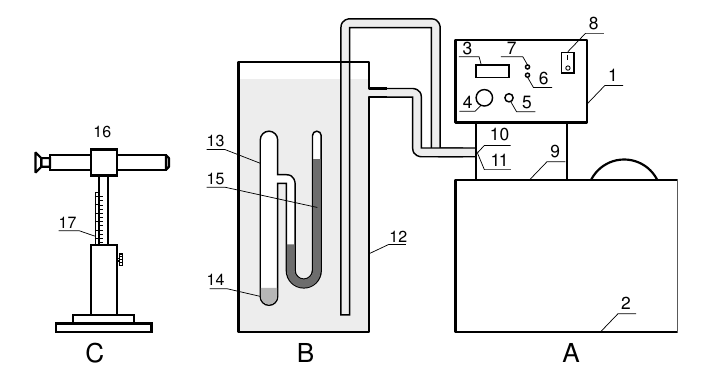
\includegraphics[scale=0.6]{scheme.png}
	\end{center}
	\end{figure}
	
	Схема установки приведена на рис. \ref{fig:scheme}. На ней показаны:
	\begin{enumerate}
		\addtocounter{enumi}{11}
		\item резвервуар с водой;
		\item запаянный прибор;
		\item исследуемая жидкость;
		\item ртутный манометр;
		\item отсчётный микроскоп;
		\item шкала штангенциркуля для снятия показаний.
	\end{enumerate}
	
	Из запаянного прибора перед погружением был удалён воздух, так что в нём находится только жидкость и её насыщенный пар. Давление снимается по разности показаний отсчётного микроскопа, настраиваемого последовательно на нижний и верхний уровни стоблика ртути манометра.
	
	Преимущество выбранного метода над прямым в том, что при непосредственном измерении требуется постоянное давление и прибор не может быть запаян, из-за чего нельзя достигнуть высокой точности.
	
	Важный недостаток установки в том, что термометр измеряет температуру термостата, а не исследуемой жидкости, поэтому нагревание должно идти достаточно медленно. Для того, чтобы проверить это, проводятся измерения при нагревании и при охлаждении жидкости в термостате.
	
	\section*{Ход работы}
	
	\begin{enumerate}
		\item Мы измерили начальную температуру ($t_0=24 ^\circ \text{C}$) и разность уровней в манометре ($h_0=2{,}05 \,\text{см}$).
		\item Включили термостат и стали постепенно нагревать воду до $t_1=50 ^\circ \text{C}$.
		\item Через каждый градус записывали разность уровней в манометре.
		\item Пустили холодную воду, охлаждая термостат до начальной температуры.
		\item Через каждый градус записывали разность уровней в манометре.
	\end{enumerate}
	
	\section*{Обработка результатов}
	
	Результаты эксперимента приведены в таблице \ref{tbl:res}.
	
	\begin{table}[!h]
	\caption{Результаты}
	\label{tbl:res}
	\begin{center}
	\begin{tabular}{|c|c|c|}
	\hline
	$t, ^\circ\text{C}$ & $h_\text{н}$, см & $h_\text{о}$, см \\
	\hline
	25 & 2.1 & 2.04 \\
	26 & 2.19 & 2.21 \\
	27 & 2.27 & 2.38 \\
	28 & 2.41 & 2.55 \\
	29 & 2.55 & 2.67 \\
	30 & 2.72 & 2.83 \\
	31 & 2.83 & 3.0 \\
	32 & 3.0 & 3.23 \\
	33 & 3.2 & 3.4 \\
	34 & 3.4 & 3.57 \\
	35 & 3.6 & 3.74 \\
	36 & 3.82 & 4.02 \\
	37 & 4.08 & 4.3 \\
	38 & 4.3 & 4.58 \\
	39 & 4.53 & 4.75 \\
	40 & 4.81 & 4.98 \\
	41 & 5.03 & 5.26 \\
	42 & 5.32 & 5.54 \\
	43 & 5.65 & 5.88 \\
	44 & 5.94 & 6.22 \\
	45 & 6.22 & 6.56 \\
	46 & 6.56 & 6.84 \\
	47 & 6.84 & 7.29 \\
	48 & 7.29 & 7.63 \\
	49 & 7.69 & 7.97 \\
	50 & 8.02 & 8.25 \\
	\hline
	\end{tabular}
	\end{center}
	\end{table}
	
	Поскольку давление, измеряемое манометром $P=\rho gh$, то $$ \ln \frac{P}{P_0} = \ln \frac{h}{h_0}. $$
	
	По снятым точкам для нагревания и охлаждения исследуемой жидкости я получил нужные логарифмы и оценил их погрешность как $$ \sigma_{\ln \left( h/h_0 \right)} = \frac{\sigma_h}{h}, $$ где $\sigma_h$ было оценено как одно деление на шкале отсчётного микроскопа (две половины, потому что отсчёт ведётся два раза), отдельно было измерено 50 дел $\approx$ 1,41 см.
	
	Экспериментальные точки для нагревания и охлаждения жидкости отдельно были аппроксимированы линейной функцией по методу наименьших квадратов с различными весами точек (по погрешностям) и нанесены на график (рис. \ref{fig:graph}) вместе с линеаризациями.
	
	\begin{figure}[!h]
	\caption{График}
	\label{fig:graph}
	\begin{center}
	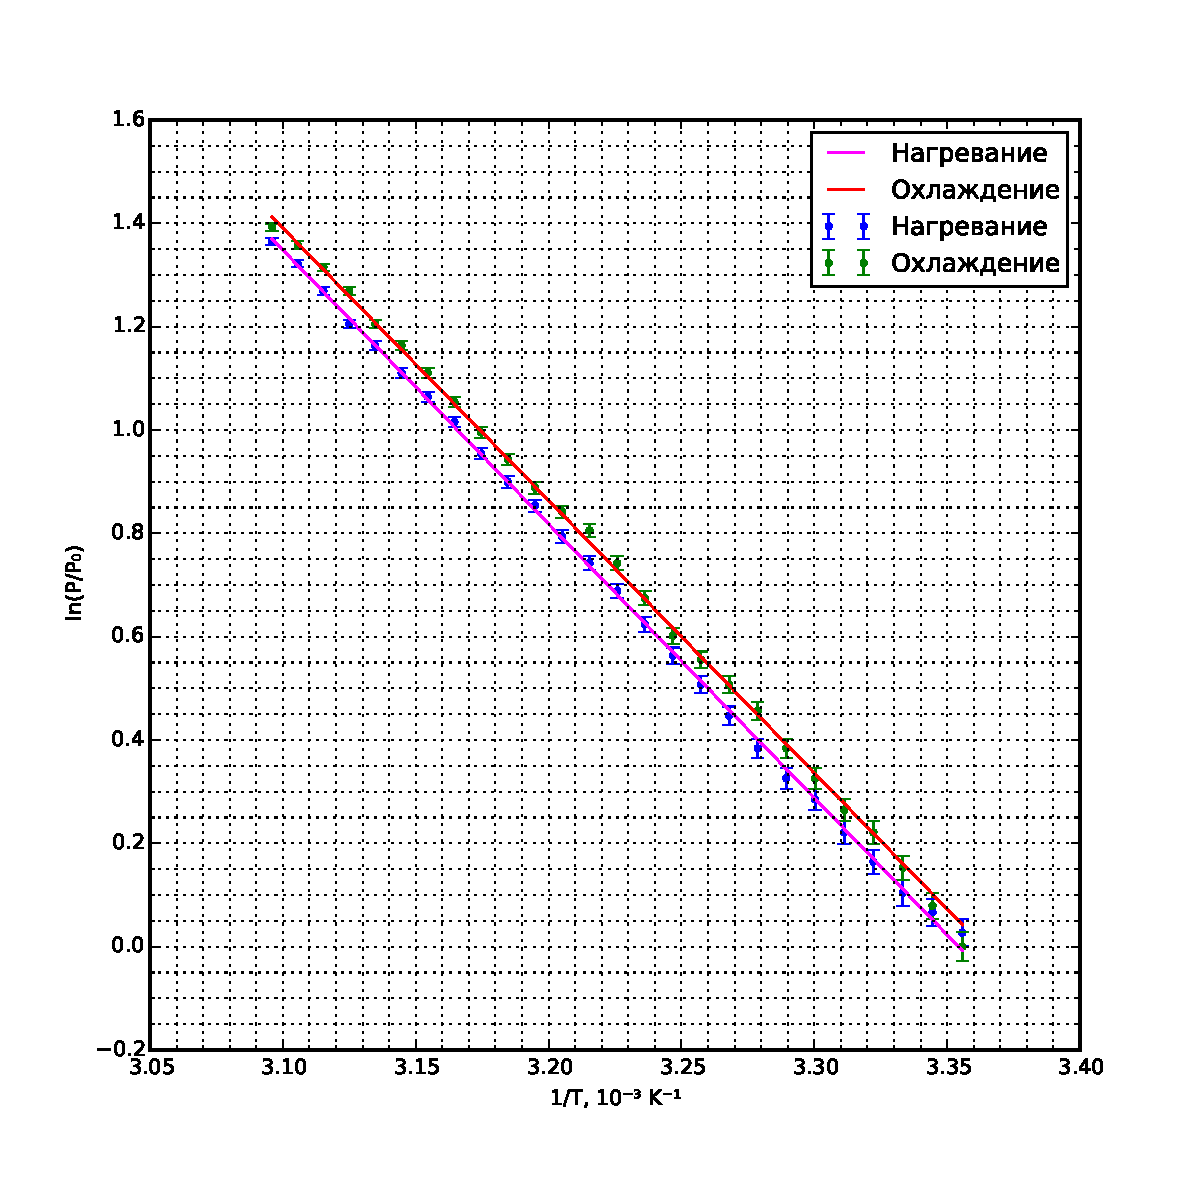
\includegraphics[scale=0.85]{graph.pdf}
	\end{center}
	\end{figure}
	
	Как мы видим, болшинство точек при охлаждении находятся чуть выше, чем при нагревании, что свидетельствует о том, что температура менялась несколько быстрее, чем следовало, из-за чего при нагревании реальная температура газа была чуть ниже, чем измеренная, а при охлаждении --- наоборот (как можно увидеть из графика или из таблицы, точки почти совпадают, только смещены на $\approx 1 ^\circ \text{C}$).
	
	Из угловых коэффициентов прямых по \eqref{eq:klapeiron-klausius_final} были вычислены молярные теплоты парообразования для кривых нагревания и охлаждения:
	$$ L_\text{н}= \left( 44{,}1 \pm 0{,}2 \right) \frac{\text{кДж}}{\text{моль}}, $$
	$$ L_\text{о}= \left( 43{,}8 \pm 0{,}3 \right) \frac{\text{кДж}}{\text{моль}}. $$
	
	Эти результаты практически сходятся в пределах погрешности.
	
	Вообще говоря, теплота парообразования зависит от температуры, хоть и не очень сильно. В справочнике (Енохович А.С. Краткий справочник по физике. М., <<Высш. школа>>, 1976) приведена удельная теплота парообразования воды при температуре $t_1=50^\circ \text{C}$ $\lambda_1=2{,}38 \frac{\text{МДж}}{\text{кг}}$, а при $t_2=20^\circ \text{C}$ --- $\lambda_2=2{,}45 \frac{\text{МДж}}{\text{кг}}$. В пересчёте на моль это соответственно $L_1= 42{,}8 \frac{\text{кДж}}{\text{моль}}$ и $L_2= 44{,}1 \frac{\text{кДж}}{\text{моль}}$. Наши экспериментальные результаты попадают в этот диапазон, что тоже свидетельствует об их адекватности.
	
\end{document}
